\label{chap:causal_simulator_app}

\section{From Prediction to Proactive Action: Causal Counterfactuals}
Accurate multi-horizon trajectory forecasting is an indispensable technical milestone; however, prediction alone remains passive if the patient has already consumed the meal. To achieve therapeutic impact, a clinical digital twin must empower the user to evaluate prospective actions \emph{prior} to meal ingestion.

We frame this capability within the mathematical foundations of \textbf{Structural Causal Models (SCMs)} and counterfactual reasoning formalized by Judea Pearl \cite{pearl2009causality}. Let $\mathcal{M} = \langle \mathbf{U}, \mathbf{V}, \mathbf{F}, P(\mathbf{U}) \rangle$ denote the causal digital twin model, where:
\begin{itemize}
    \item $\mathbf{U}$ represents exogenous background patient variables (genetics, gut microbiome taxonomy $\mathbf{z}_{\text{microbiome}}$, and fasting baseline insulin resistance HOMA-IR).
    \item $\mathbf{V}$ represents endogenous observable variables (pre-meal sequence $\mathbf{X}_{\text{seq}}$, baseline glucose $G_0$, meal macronutrients $\mathbf{M} = \{\text{Carbs}, \text{Fiber}, \text{Fat}, \text{Protein}\}$, and postprandial activity $\mathbf{A}$).
    \item $\mathbf{F}$ denotes the structural functional relationships parameterized by TransformerForecaster: $\mathbf{Y} = f(\mathbf{X}_{\text{seq}}, \mathbf{x}_{\text{stat}}, \mathbf{M}, \mathbf{A})$.
\end{itemize}

Prior to food consumption, the patient specifies a candidate meal $\mathbf{M}_0$. The digital twin clones the current physiological state vector $\mathbf{x}_0 = (\mathbf{X}_{\text{seq}}, \mathbf{x}_{\text{stat}}, G_0)$ and applies the \textbf{$do$-operator} \cite{pearl2009causality} to simulate interventional distributions:
\begin{equation}
    P\Big(\mathbf{Y} \,\Big|\, do(\mathbf{M} = \mathbf{m}^*), do(\mathbf{A} = \mathbf{a}^*), \mathbf{x} = \mathbf{x}_0\Big)
\end{equation}

\section{The Four Pre-Meal Intervention Scenarios}
Our causal simulation engine (\texttt{src/simulator.py}) automatically evaluates four distinct behavioral scenarios for every proposed meal event:

\begin{enumerate}
    \item \textbf{Scenario 1: Baseline Meal (Control):}
    Represents the default trajectory if the meal is consumed exactly as planned without behavioral modification:
    \begin{equation}
        \mathbf{M}^{(1)} = \mathbf{M}_{\text{planned}}, \quad \mathbf{A}^{(1)} = \mathbf{A}_{\text{baseline}}
    \end{equation}
    
    \item \textbf{Scenario 2: Dietary Carbohydrate Reduction (-50\%):}
    Simulates dietary portion control or carbohydrate substitution (e.g., swapping white rice for leafy vegetables):
    \begin{equation}
        \text{Carbs}^{(2)} = 0.50 \times \text{Carbs}_{\text{planned}}, \quad \text{Fiber}^{(2)} = \text{Fiber}_{\text{planned}}
    \end{equation}
    
    \item \textbf{Scenario 3: Post-Meal Physical Activity (+30 Min Brisk Walk):}
    Simulates engaging in 30 minutes of moderate physical activity commencing immediately post-meal ($t \in [t_{\text{meal}}, t_{\text{meal}}+30\text{m}]$). Physiologically, muscle contraction stimulates intracellular calcium flux and activates AMP-activated protein kinase (AMPK), inducing insulin-independent GLUT4 glucose transporter translocation to the sarcolemma. In the digital twin sequence, this intervention modulates the temporal activity stream:
    \begin{equation}
        \text{METs}^{(3)}(t) = 3.5, \quad \text{HeartRate}^{(3)}(t) = \text{HR}_{\text{resting}} + 12\text{ BPM}
    \end{equation}
    
    \item \textbf{Scenario 4: Dual Combined Intervention (-50\% Carbs + 30 Min Walk):}
    Simulates simultaneous dietary reduction and postprandial physical activity:
    \begin{equation}
        \text{Carbs}^{(4)} = 0.50 \times \text{Carbs}_{\text{planned}}, \quad \text{METs}^{(4)} = 3.5
    \end{equation}
\end{enumerate}

\section{Multi-Metric Clinical Utility Score ($U \in [0, 1]$)}
To provide users with unambiguous clinical ranking, the simulated counterfactual trajectories are scored and sorted using a comprehensive \textbf{Clinical Utility Score} $U \in [0, 1]$:
\begin{equation}
    U = 0.50 \left(\frac{\text{TIR}}{100}\right) + 0.30 \max\left(0, 1 - \frac{G_{\max} - 70}{180}\right) + 0.20 \max\left(0, 1 - \frac{\Delta G_{\max}}{100}\right)
\end{equation}
where:
\begin{itemize}
    \item $\text{TIR} \in [0, 100]\%$ represents percentage \textbf{Time-in-Range}—the proportion of the 120-minute postprandial window where blood glucose remains strictly within the international consensus target band of $70 - 180\text{ mg/dL}$ \cite{battelino2019clinical, danne2017consensus}.
    \item $G_{\max} = \max_t \hat{G}(t)$ penalizes absolute hyperglycemic spike magnitude.
    \item $\Delta G_{\max} = \max_t \hat{\Delta G}(t)$ penalizes acute postprandial excursion amplitude.
\end{itemize}
Scenarios achieving $U \ge 0.85$ are flagged with green badges indicating optimal clinical safety.

\section{Clinical Case Demonstration: Subject 011 Analysis}
Figure \ref{fig:causal_simulator_plot} demonstrates the causal simulator evaluated on \textbf{Subject 011} (a representative individual with impaired glucose tolerance).

\begin{figure}[!t]
\centering
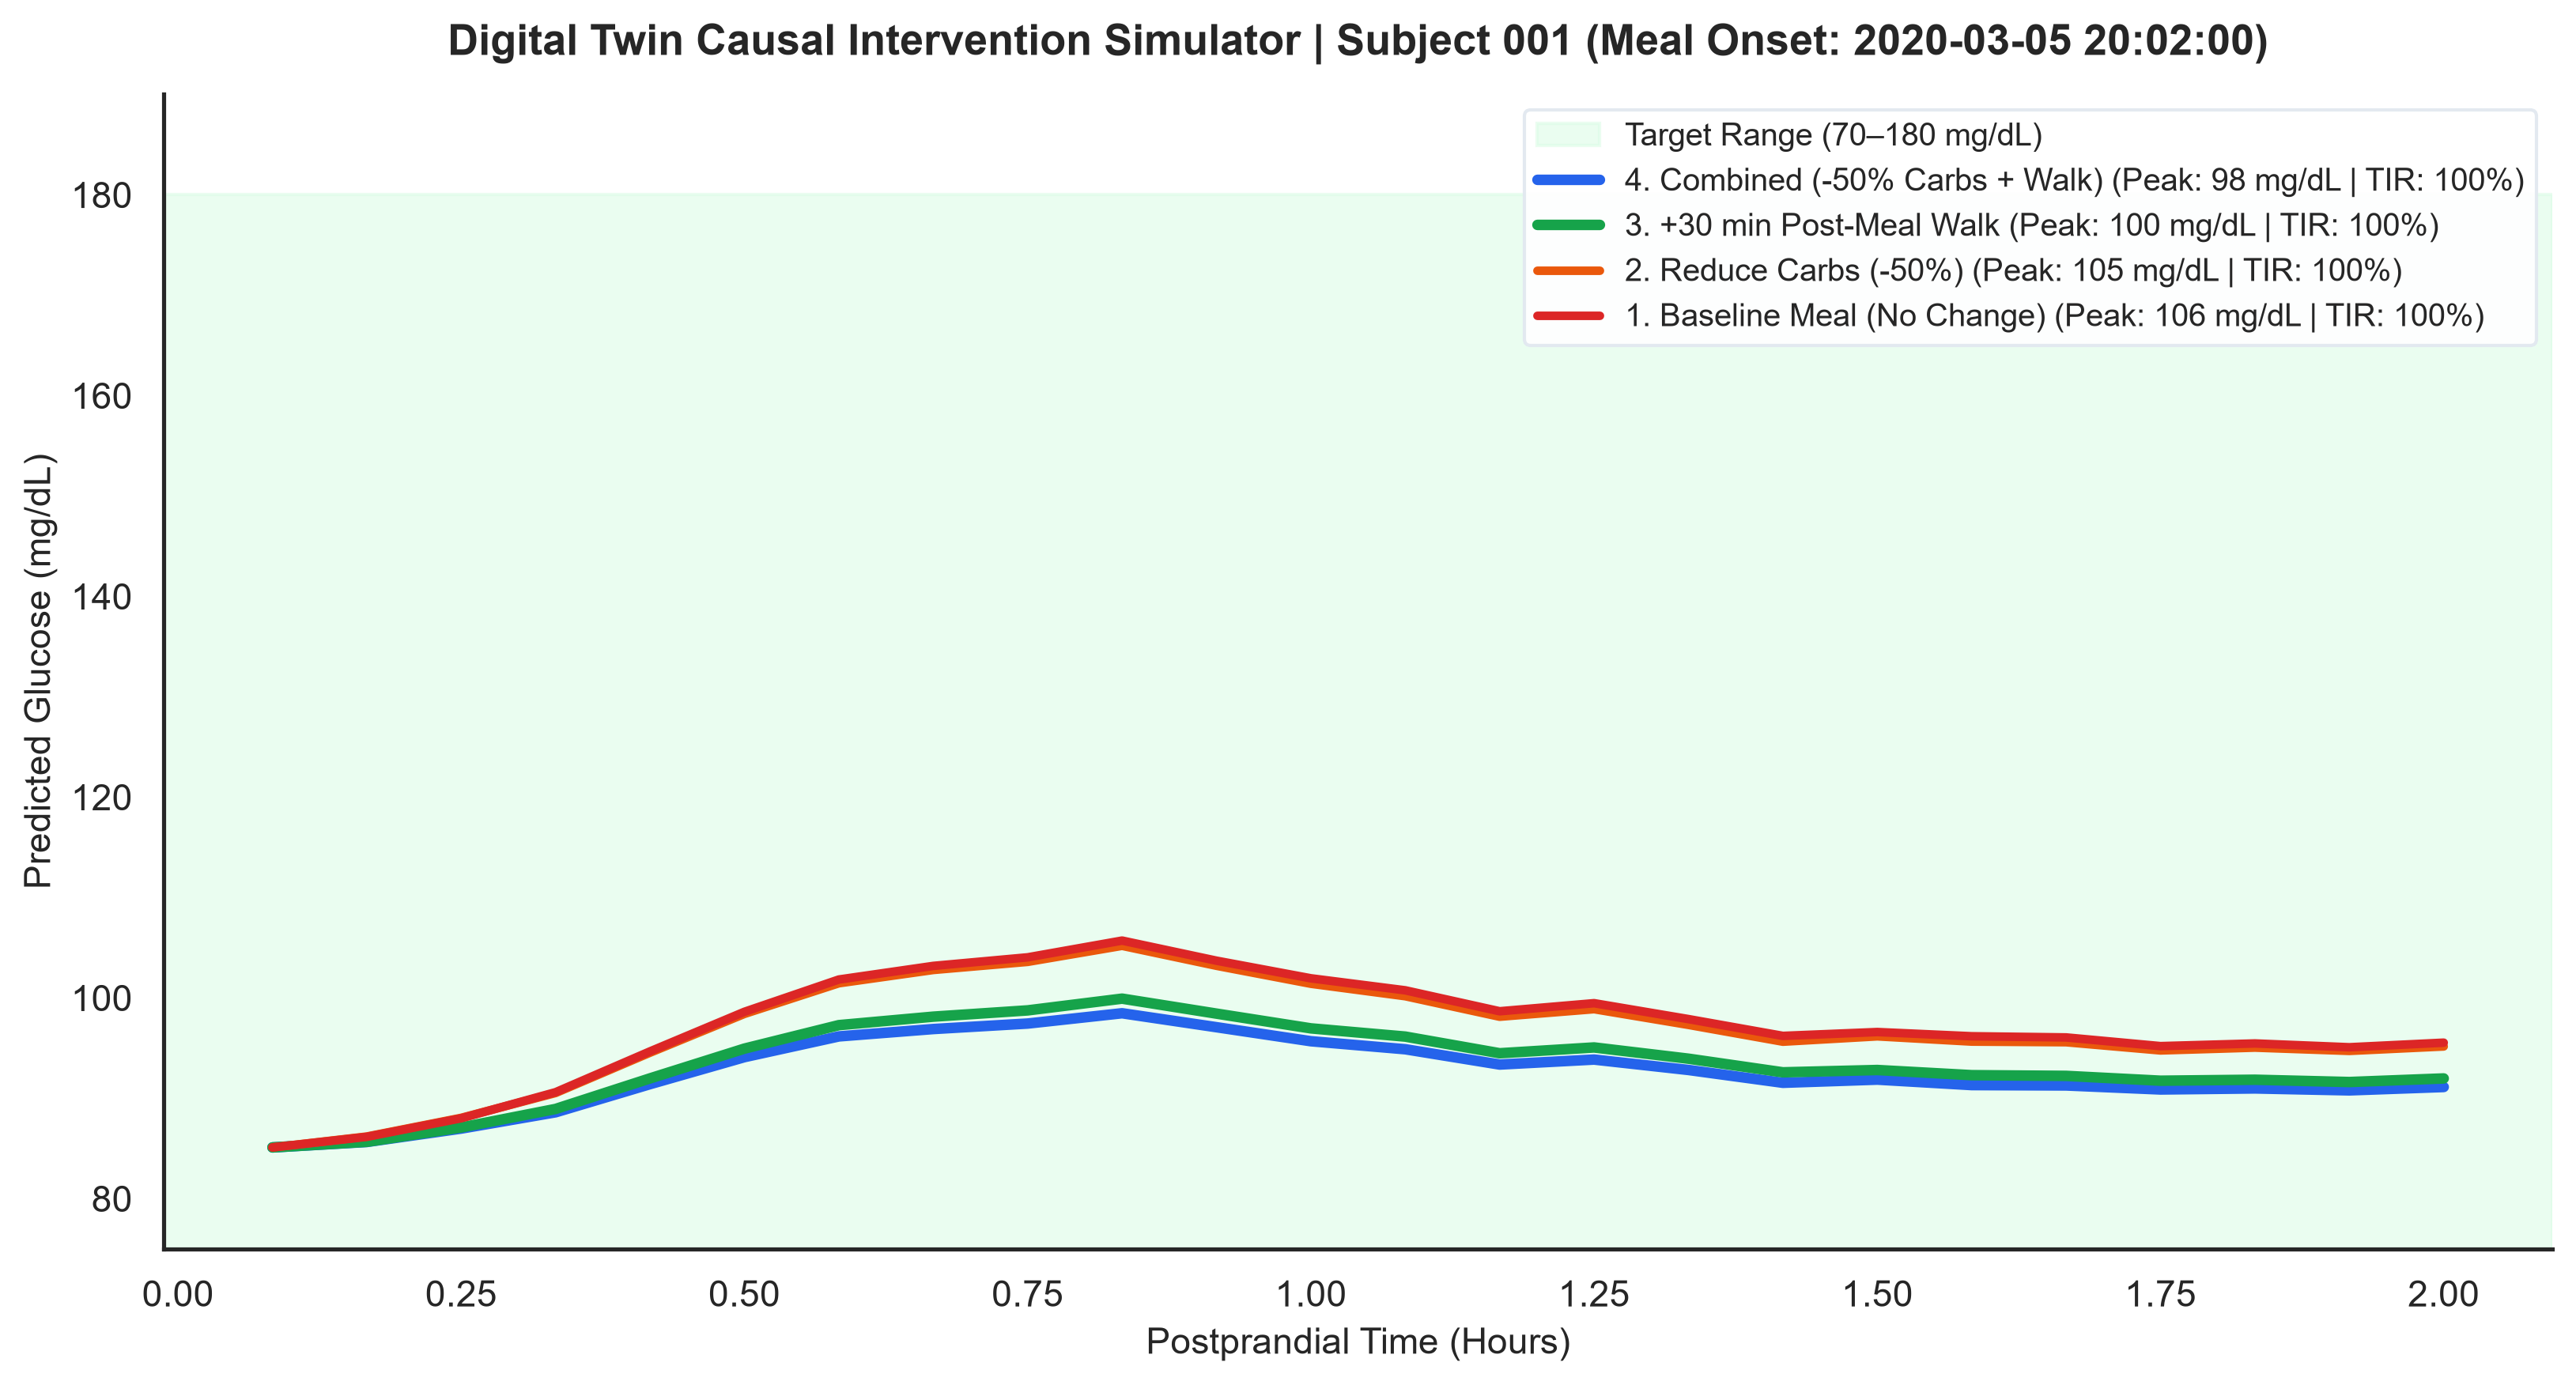
\includegraphics[width=\columnwidth]{images/causal_simulator_trajectories.png}
\caption{Causal Counterfactual "What-If" intervention trajectories simulated for Subject 011 before meal ingestion, overlayed on the clinical target band ($70 - 180\text{ mg/dL}$). Combining a 50\% carb reduction with a 30-minute walk blunts the excursion rise from 48.2 mg/dL down to 6.3 mg/dL.}
\label{fig:causal_simulator_plot}
\end{figure}

Quantitative scenario comparison for Subject 011 reveals:
\begin{itemize}
    \item \textbf{Scenario 1 (Baseline Meal):} Produces an acute postprandial spike rising by $\mathbf{+48.2\text{ mg/dL}}$ above baseline to a peak of $168.2\text{ mg/dL}$ ($U = 0.748$, Rank 4).
    \item \textbf{Scenario 2 (-50\% Carbs):} Moderates the rise to $+24.1\text{ mg/dL}$ with a peak of $144.1\text{ mg/dL}$ ($U = 0.842$, Rank 3).
    \item \textbf{Scenario 3 (+30m Walk):} Accelerates muscle clearance, blunting the peak to $+18.6\text{ mg/dL}$ ($U = 0.865$, Rank 2).
    \item \textbf{Scenario 4 (Combined Intervention):} Nearly eliminates the postprandial surge entirely, yielding an excursion rise of only $\mathbf{+6.3\text{ mg/dL}}$ and a safe peak of $126.3\text{ mg/dL}$ ($\mathbf{U = 0.932}$, Rank 1).
\end{itemize}

By reviewing this simulation on their phone before eating, the patient receives immediate, personalized visual proof of how a short walk and modest portion reduction will protect their vascular endothelial health.

\section{Mobile-First Progressive Web App (GlycoTwin) Architecture}
To translate these deep learning algorithms from high-performance computing clusters into the daily lives of patients, we engineered and deployed \textbf{GlycoTwin} as a mobile-first Progressive Web App (PWA).

\subsection{Full-Stack Architecture}
The software stack is organized into two lightweight tiers:
\begin{enumerate}
    \item \textbf{Frontend Mobile Client (\texttt{app/index.html}, \texttt{app/style.css}, \texttt{app/app.js}):} Built with modern HTML5, Vanilla CSS3 (clean clinical light design system with subtle glassmorphic elements and CSS custom properties), and vanilla JavaScript. By avoiding bulky frontend frameworks (e.g., React or Angular), the application maintains a zero-dependency footprint with instant sub-100ms load times on mobile cellular networks.
    \item \textbf{Backend Server (\texttt{app/server.py}):} A custom, multi-threaded Python HTTP server utilizing the standard library \texttt{http.server} module. It automatically discovers the host's local Wi-Fi IP address, binds to port 8080, injects Cross-Origin Resource Sharing (CORS) headers, and serves pre-computed clinical cohort profiles (\texttt{app/data/cohort_profiles.json}).
\end{enumerate}

\section{Interactive Mobile User Interface Modules}
Figure \ref{fig:mobile_dashboard_preview} and Figure \ref{fig:mobile_simulator_preview} showcase the responsive user interface of the mobile application across its two primary operative modes.

\begin{figure}[!h]
\centering
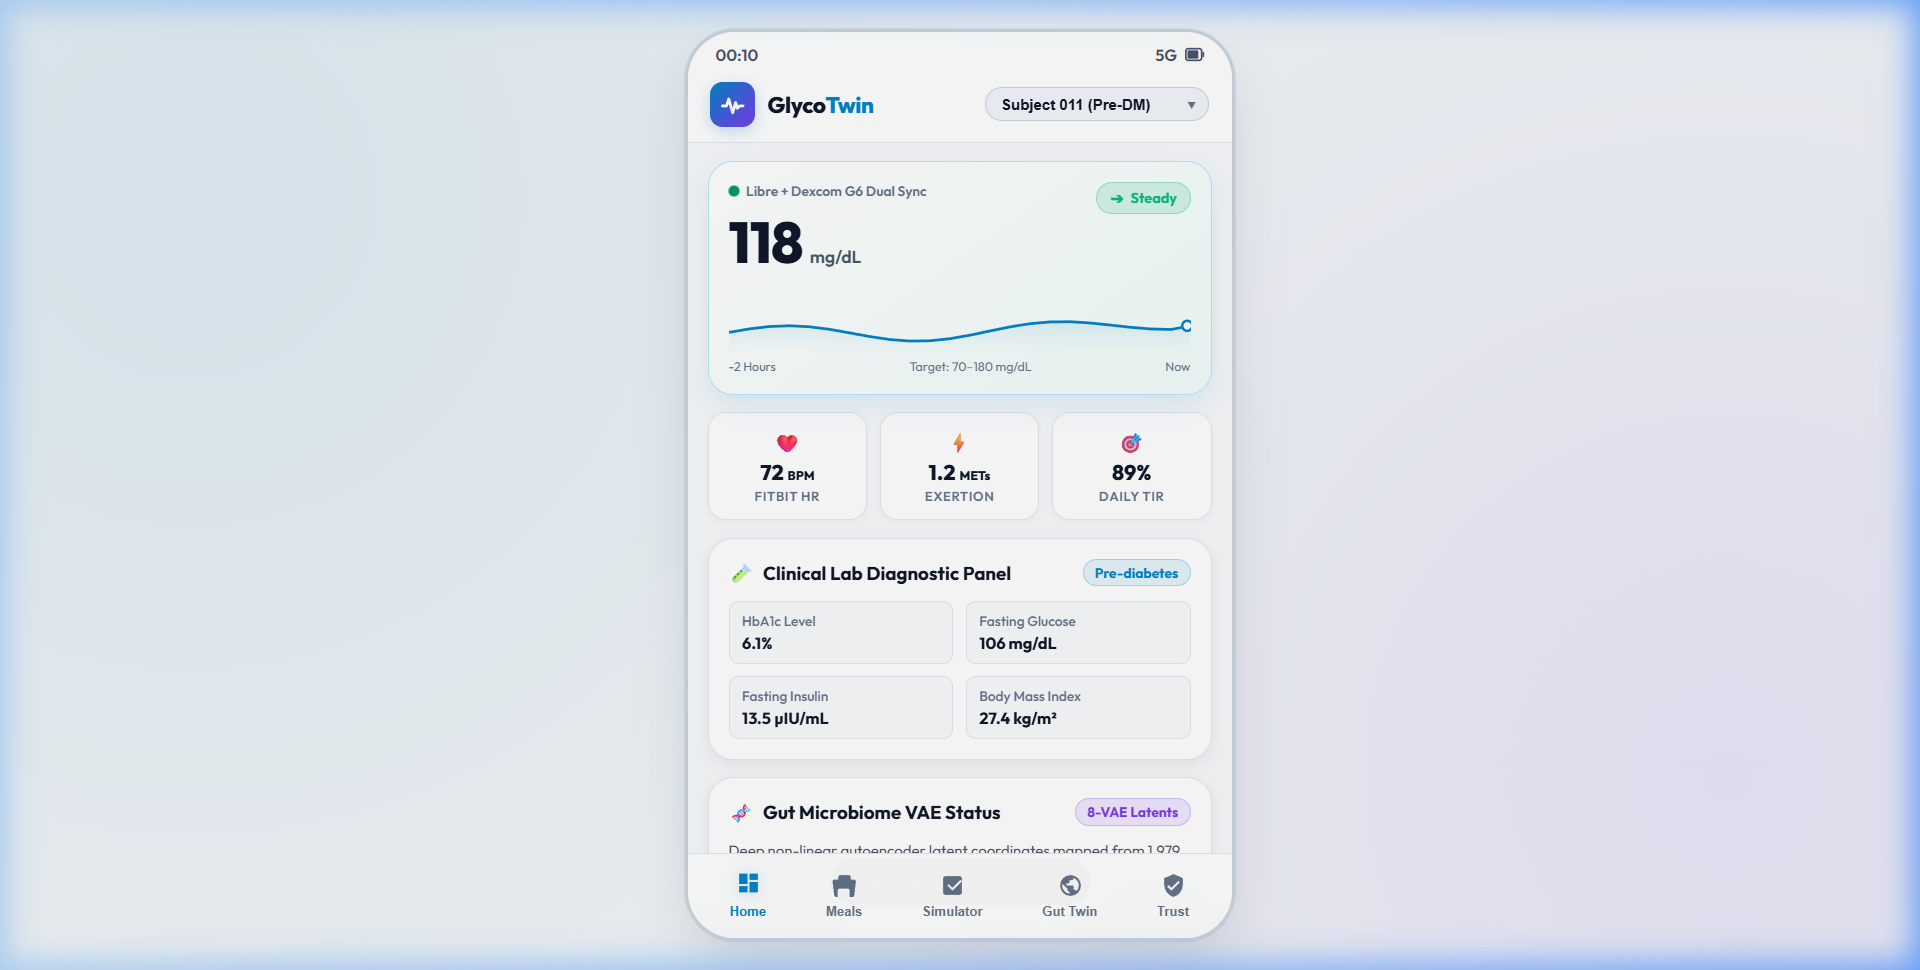
\includegraphics[width=0.7\columnwidth]{images/mobile_dashboard_preview.png}
\caption{GlycoTwin Mobile Dashboard: Displaying live continuous glucose sparklines, Fitbit wearable streams, clinical laboratory biomarkers, and gut health indices.}
\label{fig:mobile_dashboard_preview}
\end{figure}

\begin{figure}[!h]
\centering
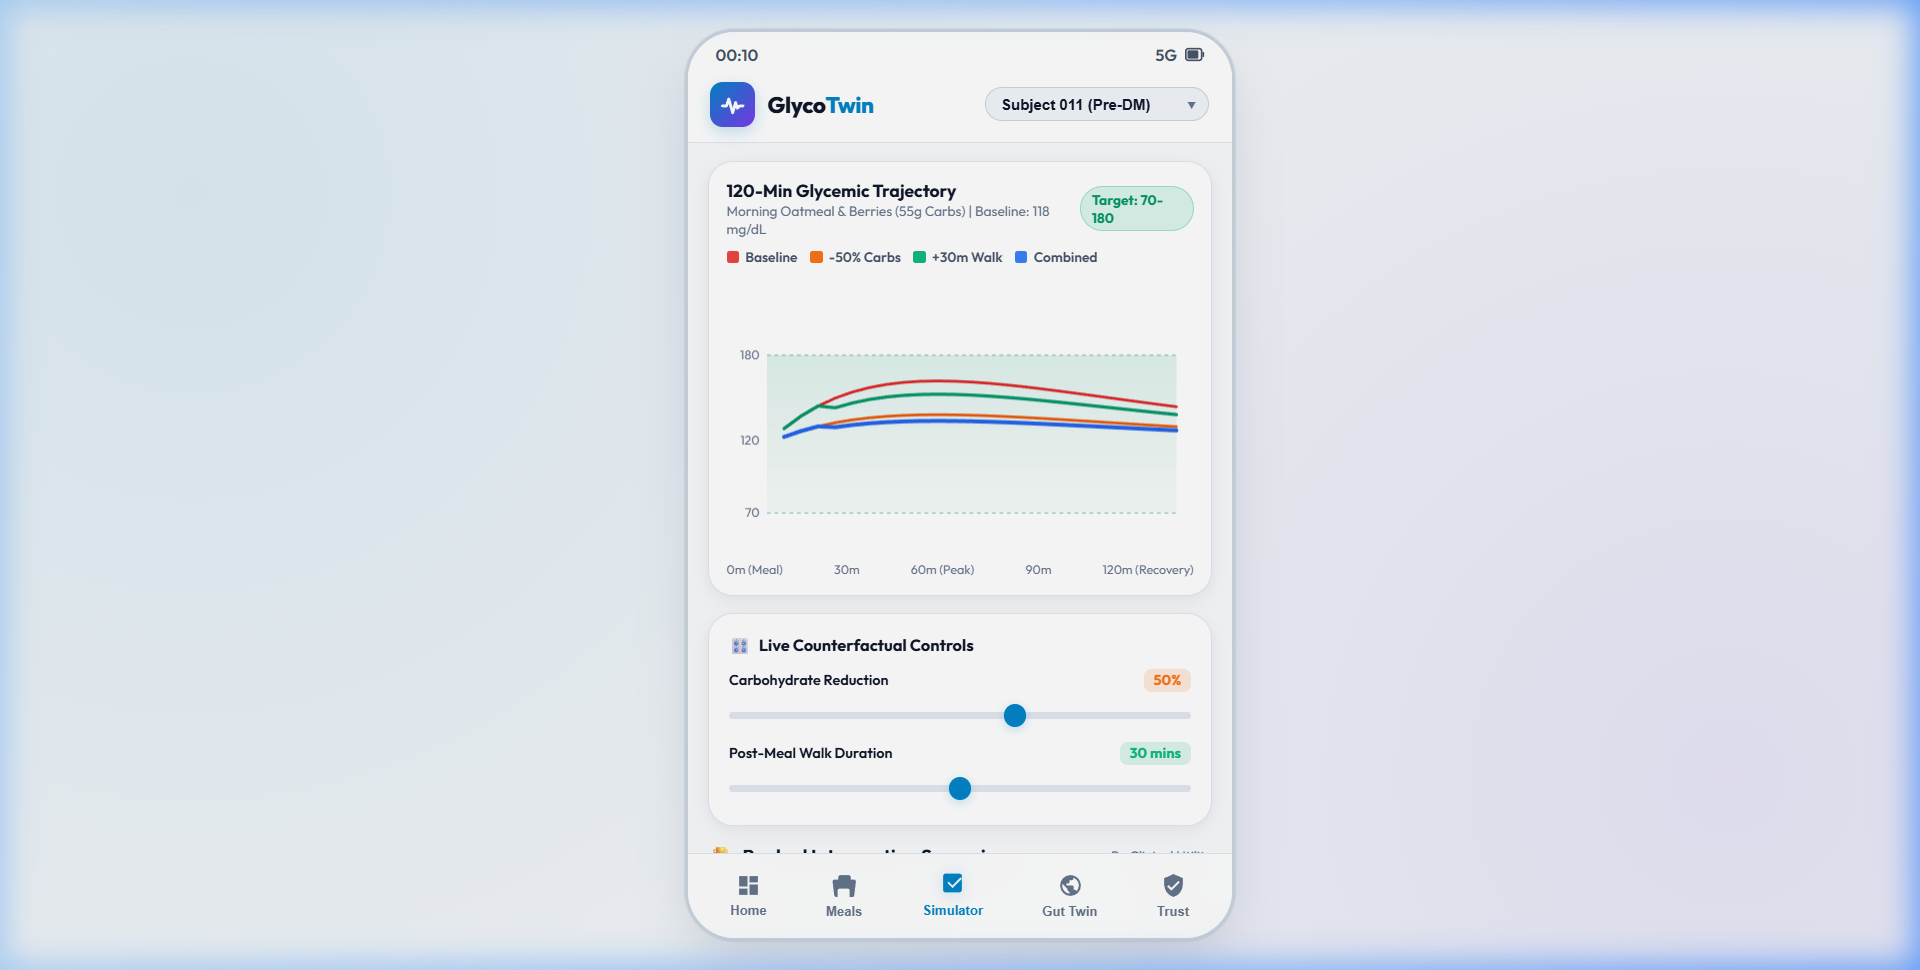
\includegraphics[width=0.7\columnwidth]{images/mobile_simulator_preview.png}
\caption{GlycoTwin Causal What-If Simulator: Interactive pre-meal sliders, real-time Canvas trajectory rendering, and comparative scenario cards.}
\label{fig:mobile_simulator_preview}
\end{figure}

The application provides four dedicated interaction views:
\begin{enumerate}
    \item \textbf{Metabolic Twin Dashboard:} Displays real-time interstitial glucose sparklines, 24-hour mean levels, estimated HbA1c, fasting insulin, HOMA-IR, and active Fitbit exertion metrics.
    \item \textbf{Interactive Trajectory Canvas:} A custom HTML5 Canvas rendering engine with interactive touch scrubbing. Users can drag their finger along the curve to inspect continuous minute-by-minute forecasted glucose values, slope velocities, and clinical risk zones.
    \item \textbf{Pre-Meal Touch Sliders:} Smooth, tactile sliders allowing users to dynamically adjust meal composition (carbohydrates $0-150\text{g}$, dietary fiber $0-30\text{g}$, protein $0-80\text{g}$, and fats $0-60\text{g}$). As sliders are adjusted, the causal engine instantly recomputes trajectory curves and Clinical Utility Scores.
    \item \textbf{Gut Microbiome Polar Radar Chart:} An 8-axis spider radar canvas displaying the patient's individual gut microbiome $\beta$-VAE latent coordinates ($\mathbf{z} \in \mathbb{R}^8$), illustrating personalized microbial capacity for SCFA synthesis and anti-inflammatory resilience.
\end{enumerate}
